%% TITLE	Physiological Fluid Mechanics, Summary 4

%% DATE		- May 17, 2022     first release
%%          - Nov 19, 2023      update

%% AUTHOR	BINGHUAN W LI (Dept. Chemical Eng/Bio Eng, Imperial)
%%          PETER Y XIE (Dept. Mech Eng, Stanford)

%% compiled in XeLaTeX with Tex Live version 2023.

%% This work is licensed under a Creative Commons Attribution-NonCommercial 4.0 International License.

\documentclass[a4paper]{article}
\newcommand{\summaryNo}{4}
%% TITLE	Physiological Fluid Mechanics, configuration

%% DATE		- Nov 19, 2023     create

%% AUTHOR	BINGHUAN W LI (Dept. Chemical Eng/Bio Eng, Imperial)
%%          PETER Y XIE (Dept. Mech Eng, Stanford)

%% compiled in XeLaTeX with Tex Live version 2023.

%% This work is licensed under a Creative Commons Attribution-NonCommercial 4.0 International License.

\usepackage[sfdefault]{arimo}
\usepackage[left=1.5cm, right=1.5cm, top=2cm, bottom=1.5cm]{geometry}
\usepackage{amsmath, amsfonts, amssymb, cancel}
\usepackage{unicode-math}
\setmathfont
    [    Extension = .otf,
         BoldFont = XITSMath-Bold,
    ]{XITSMath-Regular}

% % \DeclareMathSizes{10}{12}{10}{9}

% \usepackage{siunitx}
\usepackage{enumitem}
\usepackage{xcolor}
    \definecolor{linkcolour}{rgb}{0,0.2,0.6}
\usepackage{hyperref}
\hypersetup{
    colorlinks,
    breaklinks,
    urlcolor=linkcolour,
    linkcolor=linkcolour,
    citecolor=black,
    pdfauthor={Li, Binghuan W},
    }
\usepackage{graphicx, float}
\usepackage{framed}
\usepackage[export]{adjustbox}

\usepackage{fancyhdr}
    \pagestyle{fancy}
    \fancyhf{}
    \lhead{\textsc{Physiological Fluid Mechanics Summary \summaryNo}}
    \rhead{page \thepage}

\usepackage{tcolorbox}

\usepackage{tikz, circuitikz}

\usepackage{multicol}
    \setlength{\columnseprule}{1pt}

\usepackage{lscape}

\usepackage{booktabs}

\usepackage{pifont}

\setlength\parindent{0pt}

\begin{document}


\section{Dimensional Analysis}
\paragraph{Buckingham-$\Pi$ Theorem} The Buckingham-$\Pi$ theorem states that if an equation involving $k$ variables is dimensionally homogeneous (\textit{i.e.}, L.H.S. units = R.H.S. units), 
\[
    u_1 = f(u_2, u_3, ..., u_k),
\]
it can be reduced to a relationship among $(k-r)$ independent dimensionless products, where $r$ is the minimum number of reference dimensions required to describe the variables,
\[
    \Pi_1 = \Phi(\Pi_2, \Pi_3, ... \Pi_{k-r}).
\]

\begin{tcolorbox}[title = \textbf{Example}]
Consider the objective equation,
\[
    \Delta P_\ell = f (D, \rho, \mu, V)
\]
Let [$L$] denotes the dimension of length; [$T$] denotes the dimension of time; [$M$] denotes the dimension of mass, hence,
\begin{table}[H]
    \centering
    \begin{tabular}{ccc}
    \toprule
    $\Delta P_\ell$ &   pressure drop   &   [$ML^{-1}T^2$] \\
    \midrule
    $D$   &   pipe diameter  &   [$L$] \\
    $\rho$  &   density  & [$ML^{-3}$]\\
    $\mu$   &   dynamic viscosity   &   [$ML^{-1}T^{-1}$] \\
    $V$ &   velocity    &   [$LT^{-1}$] \\
    \bottomrule
    \end{tabular}
\end{table}
Hence we conclude $k = 5$ ($\Delta P_\ell$, $D$, $\rho$, $\mu$, $V$), $r = 3$ ($M$, $L$, $T$), we should expect $k-r = 2$ dimensionless groups.
\begin{enumerate}
    \item The first group involves $\Delta P_\ell$. Let $a$, $b$, $c$, $d$ denote 4 constants to be determined,
    \[
        D^a \rho^b V^c \Delta P_\ell^d \quad \Rightarrow \quad [] = [L]^a [ML^{-3}]^b [LT^{-1}]^c [ML^{-1}T^2]^d
    \]

    \begin{itemize}
        \item balance of $[L]$: $a - 3b + c - d = 0$
        \item balance of $[M]$: $b + d = 0$
        \item balance of $[T]$: $-c + 2d = 0$
    \end{itemize}
    This is an underdetermined problem, resulting in the following relations:
    \[
        b = -d, 
        \quad c = -2d,
        \quad a = 0.
    \]
    Hence, 
    \[
        D^0 \rho^{-d} V^{-2d} \Delta P_\ell^d = \bigg(\frac{\Delta P_\ell}{\rho V^2} \bigg)^d \quad \text{is dimensionless}, \quad \Rightarrow \boxed{\Pi_1 = \frac{\Delta P_\ell}{\rho V^2}}.   
    \]

    \item Similarly, the second term involves $\mu$, follow the same rule, this yields $\displaystyle \boxed{\Pi_2 = \frac{\mu}{\rho DV}}$, which is $1/Re$.
\end{enumerate}
\end{tcolorbox}

\section{Non-Dimensional Navier Stokes Equation}
\begin{itemize}
    \item The non-dimensionalised variables are
    \[
        \mathbf{x}^* = \frac{\mathbf{x}}{L},
        \quad \quad
        \mathbf{u}^* = \frac{\mathbf{u}}{U},
        \quad \quad
        t^* = \frac{t}{L/U},
        \quad \quad
        p^* = \frac{p}{P_0}.
    \]

    \item The dimensionless Navier-Stokes momentum equation is
     \[ 
        Re\bigg(\frac{\partial \mathbf{u^{*}}}{\partial t^{*}} + (\mathbf{u^{*}}\cdot \nabla^{*})\mathbf{u^{*}} \bigg) = -\frac{P_{0}}{\frac{\mu U}{L}}\nabla^{*} p^{*} + \nabla^{*2}\mathbf{u^{*}},
     \]
    where $\displaystyle P_{0} = \frac{\mu U}{L}\max(1,Re)$. This ensures the pressure term has the same order of magnitude as other terms, since there is no natural scaling for pressure.

    \item The dimensionless Navier-Stokes continuity equation is
     \[ \nabla^{*} \cdot \mathbf{u}^{*} = 0.\]
     
     \item One needs to consider
     \begin{enumerate}
         \item {\color{red}Small $Re$ flow}: $P_0 = \mu U/L$ and the L.H.S. eliminated,
        \[ 
            \cancelto{0}{Re\bigg(\frac{\partial \mathbf{u^{*}}}{\partial t^{*}} + (\mathbf{u^{*}}\cdot \nabla^{*})\mathbf{u^{*}} \bigg)} = -\nabla^{*} p^{*} + \nabla^{*2}\mathbf{u^{*}},
            \quad \Rightarrow \quad
            \nabla^{*} p^{*} = \nabla^{*2}\mathbf{u^{*}},
        \]
        which is known as the \textbf{Stokes equation} that can be solved analytically due to its linearity.
        
        \item {\color{red}Large $Re$ flow}: $P_0 = \rho U^2$ and the viscus term eliminated (inviscid),
        \[
            \bigg(\frac{\partial \mathbf{u^{*}}}{\partial t^{*}} + (\mathbf{u^{*}}\cdot \nabla^{*})\mathbf{u^{*}} \bigg) = -\nabla^{*} p^{*}.
        \]
        \vspace{-.6cm}
        \begin{figure}[H]
            \centering
            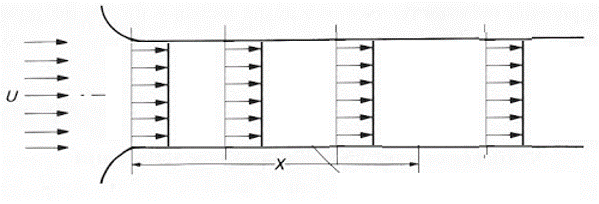
\includegraphics[width=.5\textwidth]{img/inviscid.png}
            \caption{The flow profile of the inviscid fluid. Note that the inlet flow will not develop hence the boundary layer does not exist.}
        \end{figure}
     \end{enumerate}
     
    
    % \item Lubrication Equations:
    % \[\frac{\partial u}{\partial x} + \frac{\partial v}{\partial y} = 0 
    % \quad \quad 
    % 0 = -\frac{\partial p}{\partial x} + \mu \frac{\partial^{2} u}{\partial y^{2}}\]
\end{itemize}



\section{Porous Media Flow}
\begin{itemize}
 \item Darcy Equation:\\
 \begin{minipage}{0.5\textwidth}
 \[\mathbf{u} = -\frac{k}{\mu} \nabla p\]
 \end{minipage}
 \begin{minipage}{0.4\textwidth}
    \begin{itemize}
    \begin{framed}
        \item $\mathbf{u}$ - volume flux per unit area
        \item $\mu$ - dynamic viscosity  {\color{gray}[Pa $\cdot$ s]}
        \item $k$ - permeability {\color{gray}[m\textsuperscript{2}]}
    \end{framed}
    \end{itemize}
 \end{minipage}
\end{itemize}

\section{Mass Transport}
\begin{itemize}
    \item Convection-Diffusion Equation\\
    \begin{minipage}{0.5\textwidth}
    \[ \underbrace{\frac{\partial c}{\partial t}}_{\text{rate of change}} + \underbrace{(\mathbf{u} \cdot \nabla) c}_{\text{convection}} =  \underbrace{\mathcal{D} \nabla^{2} c}_{\text{diffusion}} - \underbrace{f(c)}_{\text{consumption}} \] 
    \end{minipage}
    \begin{minipage}{0.4\textwidth}
    \begin{itemize}
    \begin{framed}
        \item[-] $c$ - concentration of solute  {\color{gray}[J/kg K]}
        \item[-] $\mathbf{u}$ - velocity vector
        \item[-] $\mathcal{D}$ - diffusion coefficient {\color{gray}[m\textsuperscript{2}/s]}
        \item[-] $f$ - consumption of solute
    \end{framed}
    \end{itemize}
    \end{minipage}

    \item Non-dimensional convection-diffusion equation
    \[
        \bigg( \frac{\Psi}{T} \bigg) \frac{\partial c^*}{\partial t^*} + \bigg( \frac{U\Psi}{L} \bigg) \mathbf{u}^* \cdot \nabla^* c^* = \bigg( \frac{\mathcal{D}\Psi}{L^2} \bigg) \nabla^{*2} c^* - \bigg( \frac{\Psi}{T} \bigg) f^* \ ,
    \]
    where the non-dimensional variables are
    \[
        \mathbf{x}^* = \frac{\mathbf{x}}{L},
        \quad \quad
        \mathbf{u}^* = \frac{\mathbf{u}}{U},
        \quad \quad
        t^* = \frac{t}{L/U},
        \quad \quad
        c^* = \frac{c}{\Psi}, 
        \quad \quad
        f^* = \frac{f}{\Psi} T.
    \]

    \item The P\'eclet number, $Pe$, is defined as the ratio of convection to diffusion,
    \[
        Pe = \frac{U\Psi}{L} \bigg/
        \frac{\mathcal{D}\Psi}{L^2} = \frac{UL}{\mathcal{D}}.
    \]

    \item Not complete enough - need to count for the \textbf{Taylor dispersion} effects $\Rightarrow$ larger diffusion coefficient.
    \[
        \mathcal{D}_{\mathrm{eff}} = \mathcal{D} \bigg(1 + \frac{Pe^2}{48} \bigg).
    \]
\end{itemize}

\thispagestyle{empty}
\newgeometry{margin=1.8cm}
\mbox{}
\vfill    
\begin{figure}[H]
    \includegraphics[right]{images/by-nc.eps}
\end{figure}
\textit{This work is licensed under a Creative Commons Attribution-NonCommercial 4.0 International License.}


\end{document}
%%  dimensional analysis https://projects.exeter.ac.uk/fluidflow/Courses/FluidDynamics3211-2/DimensionalAnalysis/dimensionalLecturese4.html